\documentclass[10pt]{article} 
\usepackage[margin=0.8in]{geometry}
\usepackage{amsmath}
\usepackage{hyperref} 
\usepackage{listings}
\usepackage{xcolor}
\usepackage{multicol}
\usepackage{graphicx}

\RequirePackage{color}
\RequirePackage{listings}

\lstdefinelanguage{Rust}{%
  sensitive%
, morecomment=[l]{//}%
, morecomment=[s]{/*}{*/}%
, moredelim=[s][{\itshape\color[rgb]{0,0,0.75}}]{\#[}{]}%
, morestring=[b]{"}%
, alsodigit={}%
, alsoother={}%
, alsoletter={!}%
%
%
% [1] reserve keywords
% [2] traits
% [3] primitive types
% [4] type and value constructors
% [5] identifier
%
, morekeywords={break, continue, else, for, if, in, loop, match, return, while}  % control flow keywords
, morekeywords={as, const, let, move, mut, ref, static}  % in the context of variables
, morekeywords={dyn, enum, fn, impl, Self, self, struct, trait, type, union, use, where}  % in the context of declarations
, morekeywords={crate, extern, mod, pub, super}  % in the context of modularisation
, morekeywords={unsafe}  % markers
, morekeywords={abstract, alignof, become, box, do, final, macro, offsetof, override, priv, proc, pure, sizeof, typeof, unsized, virtual, yield}  % reserved identifiers
%
% grep 'pub trait [A-Za-z][A-Za-z0-9]*' -r . | sed 's/^.*pub trait \([A-Za-z][A-Za-z0-9]*\).*/\1/g' | sort -u | tr '\n' ',' | sed 's/^\(.*\),$/{\1}\n/g' | sed 's/,/, /g'
, morekeywords=[2]{Add, AddAssign, Any, AsciiExt, AsInner, AsInnerMut, AsMut, AsRawFd, AsRawHandle, AsRawSocket, AsRef, Binary, BitAnd, BitAndAssign, Bitor, BitOr, BitOrAssign, BitXor, BitXorAssign, Borrow, BorrowMut, Boxed, BoxPlace, BufRead, BuildHasher, CastInto, CharExt, Clone, CoerceUnsized, CommandExt, Copy, Debug, DecodableFloat, Default, Deref, DerefMut, DirBuilderExt, DirEntryExt, Display, Div, DivAssign, DoubleEndedIterator, DoubleEndedSearcher, Drop, EnvKey, Eq, Error, ExactSizeIterator, ExitStatusExt, Extend, FileExt, FileTypeExt, Float, Fn, FnBox, FnMut, FnOnce, Freeze, From, FromInner, FromIterator, FromRawFd, FromRawHandle, FromRawSocket, FromStr, FullOps, FusedIterator, Generator, Hash, Hasher, Index, IndexMut, InPlace, Int, Into, IntoCow, IntoInner, IntoIterator, IntoRawFd, IntoRawHandle, IntoRawSocket, IsMinusOne, IsZero, Iterator, JoinHandleExt, LargeInt, LowerExp, LowerHex, MetadataExt, Mul, MulAssign, Neg, Not, Octal, OpenOptionsExt, Ord, OsStrExt, OsStringExt, Packet, PartialEq, PartialOrd, Pattern, PermissionsExt, Place, Placer, Pointer, Product, Put, RangeArgument, RawFloat, Read, Rem, RemAssign, Seek, Shl, ShlAssign, Shr, ShrAssign, Sized, SliceConcatExt, SliceExt, SliceIndex, Stats, Step, StrExt, Sub, SubAssign, Sum, Sync, TDynBenchFn, Terminal, Termination, ToOwned, ToSocketAddrs, ToString, Try, TryFrom, TryInto, UnicodeStr, Unsize, UpperExp, UpperHex, WideInt, Write}
, morekeywords=[2]{Send}  % additional traits
%
, morekeywords=[3]{bool, char, f32, f64, i8, i16, i32, i64, isize, str, u8, u16, u32, u64, unit, usize, i128, u128}  % primitive types
%
, morekeywords=[4]{Err, false, None, Ok, Some, true}  % prelude value constructors
% grep 'pub \(type\|struct\|enum\) [A-Za-z][A-Za-z0-9]*' -r . | sed 's/^.*pub \(type\|struct\|enum\) \([A-Za-z][A-Za-z0-9]*\).*/\2/g' | sort -u | tr '\n' ',' | sed 's/^\(.*\),$/{\1}\n/g' | sed 's/,/, /g'    
, morekeywords=[3]{AccessError, Adddf3, AddI128, AddoI128, AddoU128, ADDRESS, ADDRESS64, addrinfo, ADDRINFOA, AddrParseError, Addsf3, AddU128, advice, aiocb, Alignment, AllocErr, AnonPipe, Answer, Arc, Args, ArgsInnerDebug, ArgsOs, Argument, Arguments, ArgumentV1, Ashldi3, Ashlti3, Ashrdi3, Ashrti3, AssertParamIsClone, AssertParamIsCopy, AssertParamIsEq, AssertUnwindSafe, AtomicBool, AtomicPtr, Attr, auxtype, auxv, BackPlace, BacktraceContext, Barrier, BarrierWaitResult, Bencher, BenchMode, BenchSamples, BinaryHeap, BinaryHeapPlace, blkcnt, blkcnt64, blksize, BOOL, boolean, BOOLEAN, BoolTrie, BorrowError, BorrowMutError, Bound, Box, bpf, BTreeMap, BTreeSet, Bucket, BucketState, Buf, BufReader, BufWriter, Builder, BuildHasherDefault, BY, BYTE, Bytes, CannotReallocInPlace, cc, Cell, Chain, CHAR, CharIndices, CharPredicateSearcher, Chars, CharSearcher, CharsError, CharSliceSearcher, CharTryFromError, Child, ChildPipes, ChildStderr, ChildStdin, ChildStdio, ChildStdout, Chunks, ChunksMut, ciovec, clock, clockid, Cloned, cmsgcred, cmsghdr, CodePoint, Color, ColorConfig, Command, CommandEnv, Component, Components, CONDITION, condvar, Condvar, CONSOLE, CONTEXT, Count, Cow, cpu, CRITICAL, CStr, CString, CStringArray, Cursor, Cycle, CycleIter, daddr, DebugList, DebugMap, DebugSet, DebugStruct, DebugTuple, Decimal, Decoded, DecodeUtf16, DecodeUtf16Error, DecodeUtf8, DefaultEnvKey, DefaultHasher, dev, device, Difference, Digit32, DIR, DirBuilder, dircookie, dirent, dirent64, DirEntry, Discriminant, DISPATCHER, Display, Divdf3, Divdi3, Divmoddi4, Divmodsi4, Divsf3, Divsi3, Divti3, dl, Dl, Dlmalloc, Dns, DnsAnswer, DnsQuery, dqblk, Drain, DrainFilter, Dtor, Duration, DwarfReader, DWORD, DWORDLONG, DynamicLibrary, Edge, EHAction, EHContext, Elf32, Elf64, Empty, EmptyBucket, EncodeUtf16, EncodeWide, Entry, EntryPlace, Enumerate, Env, epoll, errno, Error, ErrorKind, EscapeDebug, EscapeDefault, EscapeUnicode, event, Event, eventrwflags, eventtype, ExactChunks, ExactChunksMut, EXCEPTION, Excess, ExchangeHeapSingleton, exit, exitcode, ExitStatus, Failure, fd, fdflags, fdsflags, fdstat, ff, fflags, File, FILE, FileAttr, filedelta, FileDesc, FilePermissions, filesize, filestat, FILETIME, filetype, FileType, Filter, FilterMap, Fixdfdi, Fixdfsi, Fixdfti, Fixsfdi, Fixsfsi, Fixsfti, Fixunsdfdi, Fixunsdfsi, Fixunsdfti, Fixunssfdi, Fixunssfsi, Fixunssfti, Flag, FlatMap, Floatdidf, FLOATING, Floatsidf, Floatsisf, Floattidf, Floattisf, Floatundidf, Floatunsidf, Floatunsisf, Floatuntidf, Floatuntisf, flock, ForceResult, FormatSpec, Formatted, Formatter, Fp, FpCategory, fpos, fpos64, fpreg, fpregset, FPUControlWord, Frame, FromBytesWithNulError, FromUtf16Error, FromUtf8Error, FrontPlace, fsblkcnt, fsfilcnt, fsflags, fsid, fstore, fsword, FullBucket, FullBucketMut, FullDecoded, Fuse, GapThenFull, GeneratorState, gid, glob, glob64, GlobalDlmalloc, greg, group, GROUP, Guard, GUID, Handle, HANDLE, Handler, HashMap, HashSet, Heap, HINSTANCE, HMODULE, hostent, HRESULT, id, idtype, if, ifaddrs, IMAGEHLP, Immut, in, in6, Incoming, Infallible, Initializer, ino, ino64, inode, input, InsertResult, Inspect, Instant, int16, int32, int64, int8, integer, IntermediateBox, Internal, Intersection, intmax, IntoInnerError, IntoIter, IntoStringError, intptr, InvalidSequence, iovec, ip, IpAddr, ipc, Ipv4Addr, ipv6, Ipv6Addr, Ipv6MulticastScope, Iter, IterMut, itimerspec, itimerval, jail, JoinHandle, JoinPathsError, KDHELP64, kevent, kevent64, key, Key, Keys, KV, l4, LARGE, lastlog, launchpad, Layout, Lazy, lconv, Leaf, LeafOrInternal, Lines, LinesAny, LineWriter, linger, linkcount, LinkedList, load, locale, LocalKey, LocalKeyState, Location, lock, LockResult, loff, LONG, lookup, lookupflags, LookupHost, LPBOOL, LPBY, LPBYTE, LPCSTR, LPCVOID, LPCWSTR, LPDWORD, LPFILETIME, LPHANDLE, LPOVERLAPPED, LPPROCESS, LPPROGRESS, LPSECURITY, LPSTARTUPINFO, LPSTR, LPVOID, LPWCH, LPWIN32, LPWSADATA, LPWSAPROTOCOL, LPWSTR, Lshrdi3, Lshrti3, lwpid, M128A, mach, major, Map, mcontext, Metadata, Metric, MetricMap, mflags, minor, mmsghdr, Moddi3, mode, Modsi3, Modti3, MonitorMsg, MOUNT, mprot, mq, mqd, msflags, msghdr, msginfo, msglen, msgqnum, msqid, Muldf3, Mulodi4, Mulosi4, Muloti4, Mulsf3, Multi3, Mut, Mutex, MutexGuard, MyCollection, n16, NamePadding, NativeLibBoilerplate, nfds, nl, nlink, NodeRef, NoneError, NonNull, NonZero, nthreads, NulError, OccupiedEntry, off, off64, oflags, Once, OnceState, OpenOptions, Option, Options, OptRes, Ordering, OsStr, OsString, Output, OVERLAPPED, Owned, Packet, PanicInfo, Param, ParseBoolError, ParseCharError, ParseError, ParseFloatError, ParseIntError, ParseResult, Part, passwd, Path, PathBuf, PCONDITION, PCONSOLE, Peekable, PeekMut, Permissions, PhantomData, pid, Pipes, PlaceBack, PlaceFront, PLARGE, PoisonError, pollfd, PopResult, port, Position, Powidf2, Powisf2, Prefix, PrefixComponent, PrintFormat, proc, Process, PROCESS, processentry, protoent, PSRWLOCK, pthread, ptr, ptrdiff, PVECTORED, Queue, radvisory, RandomState, Range, RangeFrom, RangeFull, RangeInclusive, RangeMut, RangeTo, RangeToInclusive, RawBucket, RawFd, RawHandle, RawPthread, RawSocket, RawTable, RawVec, Rc, ReadDir, Receiver, recv, RecvError, RecvTimeoutError, ReentrantMutex, ReentrantMutexGuard, Ref, RefCell, RefMut, REPARSE, Repeat, Result, Rev, Reverse, riflags, rights, rlim, rlim64, rlimit, rlimit64, roflags, Root, RSplit, RSplitMut, RSplitN, RSplitNMut, RUNTIME, rusage, RwLock, RWLock, RwLockReadGuard, RwLockWriteGuard, sa, SafeHash, Scan, sched, scope, sdflags, SearchResult, SearchStep, SECURITY, SeekFrom, segment, Select, SelectionResult, sem, sembuf, send, Sender, SendError, servent, sf, Shared, shmatt, shmid, ShortReader, ShouldPanic, Shutdown, siflags, sigaction, SigAction, sigevent, sighandler, siginfo, Sign, signal, signalfd, SignalToken, sigset, sigval, Sink, SipHasher, SipHasher13, SipHasher24, size, SIZE, Skip, SkipWhile, Slice, SmallBoolTrie, sockaddr, SOCKADDR, sockcred, Socket, SOCKET, SocketAddr, SocketAddrV4, SocketAddrV6, socklen, speed, Splice, Split, SplitMut, SplitN, SplitNMut, SplitPaths, SplitWhitespace, spwd, SRWLOCK, ssize, stack, STACKFRAME64, StartResult, STARTUPINFO, stat, Stat, stat64, statfs, statfs64, StaticKey, statvfs, StatVfs, statvfs64, Stderr, StderrLock, StderrTerminal, Stdin, StdinLock, Stdio, StdioPipes, Stdout, StdoutLock, StdoutTerminal, StepBy, String, StripPrefixError, StrSearcher, subclockflags, Subdf3, SubI128, SuboI128, SuboU128, subrwflags, subscription, Subsf3, SubU128, Summary, suseconds, SYMBOL, SYMBOLIC, SymmetricDifference, SyncSender, sysinfo, System, SystemTime, SystemTimeError, Take, TakeWhile, tcb, tcflag, TcpListener, TcpStream, TempDir, TermInfo, TerminfoTerminal, termios, termios2, TestDesc, TestDescAndFn, TestEvent, TestFn, TestName, TestOpts, TestResult, Thread, threadattr, threadentry, ThreadId, tid, time, time64, timespec, TimeSpec, timestamp, timeval, timeval32, timezone, tm, tms, ToLowercase, ToUppercase, TraitObject, TryFromIntError, TryFromSliceError, TryIter, TryLockError, TryLockResult, TryRecvError, TrySendError, TypeId, U64x2, ucontext, ucred, Udivdi3, Udivmoddi4, Udivmodsi4, Udivmodti4, Udivsi3, Udivti3, UdpSocket, uid, UINT, uint16, uint32, uint64, uint8, uintmax, uintptr, ulflags, ULONG, ULONGLONG, Umoddi3, Umodsi3, Umodti3, UnicodeVersion, Union, Unique, UnixDatagram, UnixListener, UnixStream, Unpacked, UnsafeCell, UNWIND, UpgradeResult, useconds, user, userdata, USHORT, Utf16Encoder, Utf8Error, Utf8Lossy, Utf8LossyChunk, Utf8LossyChunksIter, utimbuf, utmp, utmpx, utsname, uuid, VacantEntry, Values, ValuesMut, VarError, Variables, Vars, VarsOs, Vec, VecDeque, vm, Void, WaitTimeoutResult, WaitToken, wchar, WCHAR, Weak, whence, WIN32, WinConsole, Windows, WindowsEnvKey, winsize, WORD, Wrapping, wrlen, WSADATA, WSAPROTOCOL, WSAPROTOCOLCHAIN, Wtf8, Wtf8Buf, Wtf8CodePoints, xsw, xucred, Zip, zx}
%
, morekeywords=[5]{assert!, assert_eq!, assert_ne!, cfg!, column!, compile_error!, concat!, concat_idents!, debug_assert!, debug_assert_eq!, debug_assert_ne!, env!, eprint!, eprintln!, file!, format!, format_args!, include!, include_bytes!, include_str!, line!, module_path!, option_env!, panic!, print!, println!, select!, stringify!, thread_local!, try!, unimplemented!, unreachable!, vec!, write!, writeln!}  % prelude macros
}%

\lstdefinestyle{colouredRust}%
{ basicstyle=\ttfamily%
, identifierstyle=%
, commentstyle=\color[gray]{0.4}%
, stringstyle=\color[rgb]{0, 0, 0.5}%
, keywordstyle=\bfseries% reserved keywords
, keywordstyle=[2]\color[rgb]{0.75, 0, 0}% traits
, keywordstyle=[3]\color[rgb]{0, 0.5, 0}% primitive types
, keywordstyle=[4]\color[rgb]{0, 0.5, 0}% type and value constructors
, keywordstyle=[5]\color[rgb]{0, 0, 0.75}% macros
, columns=spaceflexible%
, keepspaces=true%
, showspaces=false%
, showtabs=false%
, showstringspaces=true%
}%

\lstdefinestyle{boxed}{
  style=colouredRust%
, numbers=left%
, firstnumber=auto%
, numberblanklines=true%
, frame=trbL%
, numberstyle=\tiny%
, frame=leftline%
, numbersep=7pt%
, framesep=5pt%
, framerule=10pt%
, xleftmargin=15pt%
, backgroundcolor=\color[gray]{0.97}%
, rulecolor=\color[gray]{0.90}%
}

\title{GxHash: A High-Throughput, Non-Cryptographic Hashing Algorithm Leveraging Modern CPU Capabilities}
\author{Olivier Giniaux}
\date{}

\begin{document}

\maketitle

\begin{abstract}

In the rapidly evolving landscape of data processing and cybersecurity, hashing algorithms play a pivotal role in ensuring data integrity and security.
Traditional hashing methods, while effective, often fail to fully utilize the computational capabilities of modern processors.
This paper introduces the GxHash hashing algorithm, a novel approach that harnesses the power of high instruction-level parallelism (ILP) and Single
Instruction, Multiple Data (SIMD) capabilities of contemporary CPUs to achieve high-throughput non-cryptographic hashing. Through a comprehensive
analysis, including benchmarks and comparisons with existing methods, we demonstrate that GxHash significantly outperforms conventional algorithms
in terms of speed and computational efficiency without compromising on security. The paper also explores the implications, limitations, and avenues
for future research in this burgeoning field.

\end{abstract}

\begin{multicols}{2}
\tableofcontents
\end{multicols}

\clearpage
\section{Introduction}

\subsection{Motivations}

As a software engineer at Equativ, a company specializing in high-performance AdServing backends that handle billions of auctions daily,
I face unique challenges in maximizing throughput while minimizing latency. In this high-stakes environment, every millisecond counts,
and the performance of underlying data structures becomes critically important. We heavily rely on in-memory caches and other hash-based data structures,
making the efficiency of hashing algorithms a non-trivial concern in our system's overall performance.\\\\
While diving into the theory of hashing out of both necessity and intellectual curiosity, I discovered that existing hashing algorithms,
including those built on well-known constructions like Merkle–Damgård, are not optimized to exploit the full capabilities of modern general-purpose CPUs.
These CPUs offer advanced features such as Single Instruction, Multiple Data (SIMD) and Instruction-Level Parallelism (ILP), which remain largely untapped
by current hashing methods.\\\\
The challenge of creating a faster, more efficient hashing algorithm became not just a professional necessity but also a personal quest.
It was both challenging and exhilarating to delve into hashing theory and experiment with new approaches. The result is what I believe to be the fastest
non-cryptographic hashing algorithm developed to date.\\\\
The primary motivation behind this research is to bridge the existing performance gap by designing a hashing algorithm that fully leverages SIMD and ILP
capabilities. The aim is to achieve an order-of-magnitude improvement in hashing speed, thereby revolutionizing the efficiency of various applications,
from databases to real-time analytics and beyond.\\\\
In summary, this work is driven by both the practical needs of my professional environment and a personal passion for pushing the boundaries of what is
technically possible in the realm of hashing algorithms.

\section{Related Work}

The field of hashing algorithms has been a subject of extensive research and development, tracing its roots back to foundational architectures like
the \textbf{Merkle–Damgård} Construction\cite{merkle}\cite{damgard}, introduced in 1989. Over the years, this area has seen a plethora of innovations, each attempting to address various
aspects of hashing—be it collision resistance, distribution uniformity, or computational efficiency. While cryptographic hashing has often been the focal
point of research, non-cryptographic hashing algorithms have also garnered attention for their utility in data structures like hashmaps and caches.

In this section, we will explore some of the seminal works and recent advancements in the realm of hashing algorithms to contextualize
our research.

\subsection{The Merkle–Damgård Construction}

The Merkle–Damgård construction serves as the foundational architecture for many existing hash functions.
It operates by breaking down an input into fixed-size blocks, which are then processed sequentially through a compression
function. The output of each block feeds into the next, culminating in a final, fixed-size hash.\\\\

Let \( h: \{0,1\}^{n_b \times s_b} \to \{0,1\}^{s_h} \) be a cryptographic hash function where: 
\begin{itemize}
    \item Input \( M \) is a binary message composed of \( n_b \) blocks of size \( s_b \),
    such as \( M = M_1 \parallel M_2 \parallel \ldots \parallel M_{n_b} \).
    \item Output is a binary hash of size \( s_h \).
\end{itemize}

The Merkle–Damgård construction can be formalized like so. Given:
\begin{itemize}
    \item The compression function \( f: \{0,1\}^{s_b} \times \{0,1\}^{s_b} \to \{0,1\}^{s_b} \)
    \item The pipe function \( g: \{0,1\}^{s_b} \to \{0,1\}^{s_h} \)
    \item A zero-filled vector \( 0^{s_b} \) of length \( s_b \)
\end{itemize}
The hash function \( h \) can be expressed as:
\begin{align*}
    h(M) &= g\left( f(\ldots f(f(0^{s_b}, M_1), M_2) \ldots, M_{n_b}) \right)
\end{align*}

\begin{figure}[h]
\centering
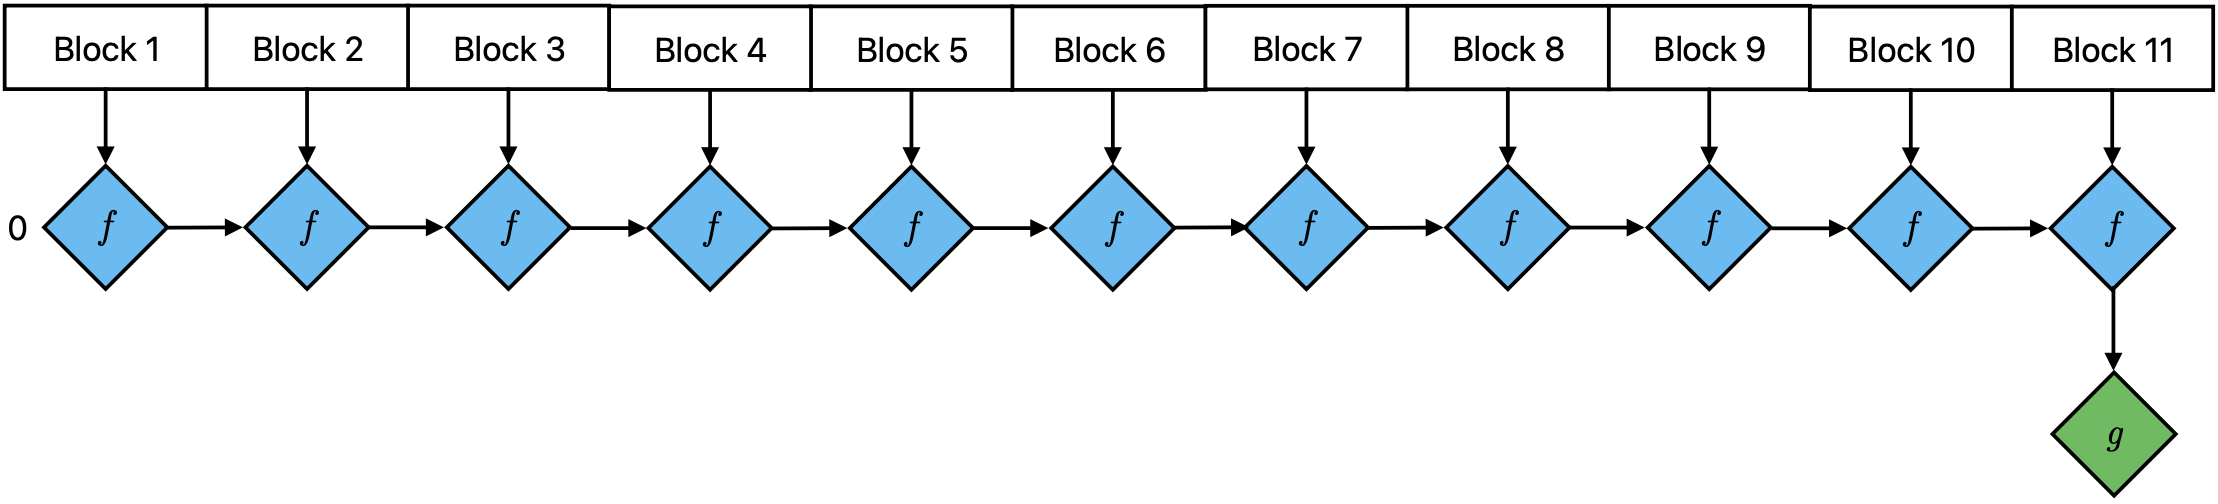
\includegraphics[width=1\textwidth]{linear-construction.png}
\caption{Merkle–Damgård Construction Overview}
\label{fig:linear-construction}
\end{figure}

\subsection{The Wide-Pipe Construction} \label{widepipe}

The \textbf{Merkle–Damgård} construction has certain limitations, such as susceptibility to length extension and multicollision attacks.
To address these issues, a variant known as the \textbf{wide-pipe} construction was introduced.
This construction employs a larger internal state, so that:
\begin{align*}
    s_b \gg s_h
\end{align*}
By taking in a larger internal chaining value, the algorithm strengthens the integrity of the hash function,
making it more challenging to reverse-engineer or compromise.

\subsection{Alternatives}

\cite{merkle_damgard_alternatives_review}

\clearpage
\section{High ILP Construction} \label{highilp}

Most modern general-purpose CPUs employ a superscalar architecture which enables Instruction-Level Parallelism (ILP). 
Minimizing dependencies in an algorithm allows a superscalar processor to execute more instructions concurrently,
thus maximizing its inherent parallelism and overall performance.
The key limitation for ILP in the Merkle–Damgård construction is the inherent sequential dependency:
each block's hash depends on the result of hashing the previous block.

\subsection{ILP Awareness}

While compilers and CPUs employ various techniques to optimize ILP, their capabilities are often constrained by the inherent data dependencies
in the code. It's for this reason that algorithmic design can be pivotal. By structuring algorithms to minimize dependency chains from the outset,
we create opportunities for higher ILP that even the most advanced compiler optimizations and CPU features cannot achieve alone. Therefore,
algorithmic design that is mindful of ILP can be a game-changer for performance optimization.

\subsubsection{Example}
Let's take a FNV-like hashing function. The "naive" way to process an array of elements would look like the \texttt{baseline} method,
as shown in Rust snippet (Figure~\ref{fig:ilp_rust_example}). As we can see, every loop iteration requires the value of \texttt{h},
which has been computed the iteration before. Here we have a dependency chain, preventing the compiler from doing any optimization.

To make ILP possible, for the function \texttt{temp} we unroll the loop and hash a few inputs altogether, independently from \texttt{h},
and mix it once thereafter with \texttt{h}. We still have a dependency chain on \texttt{h}, but for less iterations.
The temporary hashes are independent and thus eligible for ILP.

Another track taken for the function \texttt{laned} is to unroll the loop and hash on separate lanes,
and then mix the lanes together upon exiting the loop. Each lane has its own dependency chain, but on less iterations.

\begin{figure}[ht]
\begin{multicols}{2}
\begin{lstlisting}[language=Rust, style=boxed]
const PRIME: u64 = 0x00000100000001b3;
const OFFSET: u64 = 0xcbf29ce484222325;

#[inline]
fn hash(hash: u64, value: u64) -> u64 {
    (hash ^ value) * PRIME
}

fn baseline(input: &[u64]) -> u64 {
    let mut h = OFFSET;
    let mut i: usize = 0;
    while i < input.len() {
        h = hash(h, input[i]);

        i = i + 1;
    }
    h
}

fn unrolled(input: &[u64]) -> u64 {
    let mut h: u64 = OFFSET;
    let mut i: usize = 0;
    while i < input.len() {
        h = hash(h, input[i]);
        h = hash(h, input[i + 1]);
        h = hash(h, input[i + 2]);
        h = hash(h, input[i + 3]);
        h = hash(h, input[i + 4]);

        i = i + 5;
    }
    h
}
\end{lstlisting}
\columnbreak
\begin{lstlisting}[language=Rust, style=boxed]
fn temp(input: &[u64]) -> u64 {
    let mut h: u64 = OFFSET;
    let mut i: usize = 0;
    while i < input.len() {
        let mut tmp: u64 = input[i];
        tmp = hash(tmp, input[i + 1]);
        tmp = hash(tmp, input[i + 2]);
        tmp = hash(tmp, input[i + 3]);
        tmp = hash(tmp, input[i + 4]);

        h = hash(h, tmp);

        i = i + 5;
    }
    h
}

fn laned(input: &[u64]) -> u64 {
    let mut h1: u64 = OFFSET;
    let mut h2: u64 = OFFSET;
    let mut h3: u64 = OFFSET;
    let mut h4: u64 = OFFSET;
    let mut h5: u64 = OFFSET; 
    let mut i: usize = 0;
    while i < input.len() {
        h1 = hash(h1, input[i]);
        h2 = hash(h2, input[i + 1]);
        h3 = hash(h3, input[i + 2]);
        h4 = hash(h4, input[i + 3]);
        h5 = hash(h5, input[i + 4]);

        i = i + 5;
    }
    hash(hash(hash(hash(h1, h2), h3), h4), h5)
}
\end{lstlisting}
\end{multicols}
\caption{FNV-like hash functions in Rust}
\label{fig:ilp_rust_example}
\end{figure}

\clearpage
\subsubsection{Benchmark}
Here are the timing on both an x86 and an ARM CPU. It also includes timing for the function \texttt{unrolled},
to show that performance increase comes indeed from ILP and not the loop unrolling itself.
We can see that \texttt{temp} and \texttt{laned} performed equally, leveraging ILP for a significant performance increase over the \texttt{baseline}.
\\
\begin{figure}[ht]
\centering
\begin{tabular}{|c|c|c|c|c|}
\hline
CPU & \texttt{baseline} & \texttt{unrolled} & \texttt{temp} & \texttt{laned} \\
\hline
AMD Ryzen 5 5625U (x86 64-bit) & 92.787 µs & 93.047 µs & 37.516 µs & 37.434 µs \\
Apple M1 Pro (ARM 64-bit) & 125.23 µs & 124.42 µs & 28.507 µs & 30.716 µs \\
\hline
\end{tabular}
\caption{Benchmark timings for ILP example}
\label{tab:your_table_label}
\end{figure}
\\
While the \texttt{temp} and \texttt{laned} functions won't yield exactly the same hashes as the \texttt{baseline},
they serve the same purpose, while being much faster.
Both approaches have they pro and cons. As the \texttt{laned} explicitely declares \( n \) variables for our lanes,
this approach is simpler in regards to compiler analysis and is thus more likely to benefit from ILP,
regardless of the compiler or programming language used.
The following section will delve more in depth onto the definition of a \textbf{Laned Construction}.

\clearpage
\subsection{The Laned Construction}

The \textbf{Laned Construction} introduces \( k_b \) lanes, and processes the message by groups of \( k_b \) blocks,
so that for a given group each of the \( k_b \) block and be processed on its own lane.
This way, we have \( k_b \) independent dependency chains. The lane hashes can then be compressed altogether thereafter upon exiting the loop.

\subsubsection{Intermediate Hashes}

Let's define \( n_g = \lfloor {n_b}/{k_b} \rfloor \) as the number of whole groups of \( k_b \) message blocks. \\
For each lane we compute an intermediate hash, \( H_i \), as follows:

\begin{align*}
H_{1} &= f(\ldots f(f(f(0^{s_b}, M_{0k_b + 1}), M_{1k_b + 1}), M_{2k_b + 1})\ldots, M_{n_g + 1}) \\
H_{2} &= f(\ldots f(f(f(0^{s_b}, M_{0k_b + 2}), M_{1k_b + 2}), M_{2k_b + 2})\ldots, M_{n_g + 2}) \\
&\vdots \\
H_{k_b} &= f(\ldots f(f(f(0^{s_b}, M_{0k_b + k_b}), M_{1k_b + k_b}), M_{2k_b + k_b})\ldots, M_{n_g + k_b}) \\
\end{align*}

\subsubsection{Final Hash}

The final hash \( H \) is calculated using \( f \) to compress the intermediate hashes and the remaining message blocks (if any),
which is then passed through \( g \):

\begin{equation*}
h(M) = g\left( f( \ldots f(f(\ldots f(f(0^{s_b}, H_1), H_2) \ldots, H_{k_b}), M_{{k_b}{n_g}+1}) \ldots, M_{n_b} ) \right).
\end{equation*}

\begin{figure}[h]
\centering
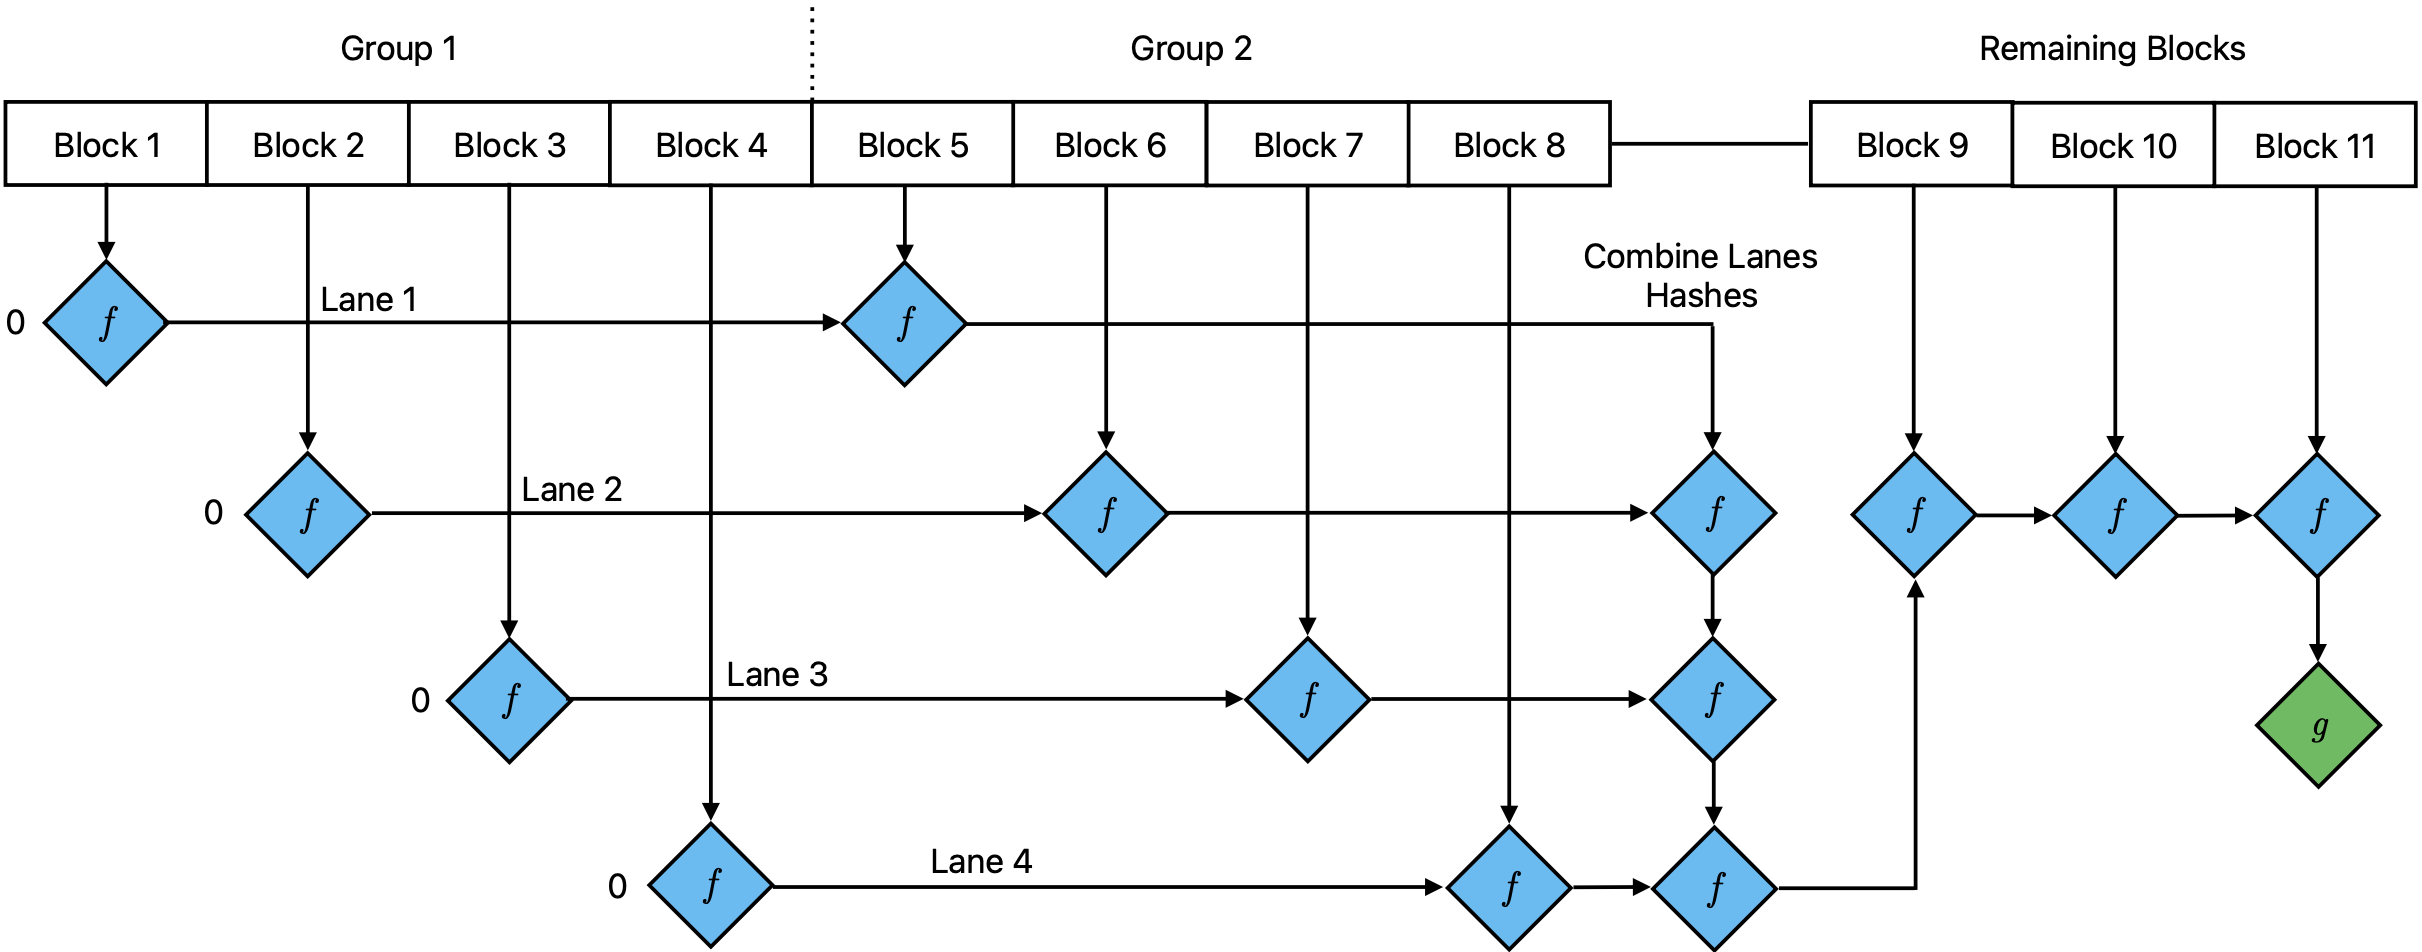
\includegraphics[width=1\textwidth]{laned-construction.png}
\caption{Laned Construction Overview}
\label{fig:linear-construction}
\end{figure}

\section{The GxHash Algorithm}

The \textbf{GxHash} hashing algorithm employs an high ILP construction as described in section \ref{highilp}. In practice,
this construction not only enables instruction level paralellism but also enables loop unrolling, disminishing the looping overhead,
thus maximizing computational efficiency and overall performance. 

\subsection{Pipe Width}
As for the wide-pipe construction (as seen in section \ref{widepipe}) with \( s_b \) set to the executing CPU SIMD register size.
TODO

\subsection{Compression}

TODO

\subsection{Hashing}

TODO

\subsection{Folding}

TODO

\subsection{Implementation Details}

SIMD
ILP
Vectorized
Parallelized
Optimized
Throughput
Hashing

HIGH ILP CONSTRUCTION

\subsubsection{Padding}

\subsubsection{Low-Overhead Looping}

\subsubsection{Loop Unrolling}

\subsubsection{CPU Alignement}

\textbf{Merkle–Damgård} and derivatives can actually handle message of an arbitrary size \( s_m \) by padding the message upfront with the padding
function \( p: \{0,1\}^{s_m} \to \{0,1\}^{n_b \times s_b} \) where \( n_b = \lceil s_m/s_b \rceil \).

In practice, implementing \( p \) in computer code implies memory copies. Instead, TODO

\section{Benchmarks}
\subsection{Setup}
\subsection{Evaluation Metrics}
\subsection{Comparison with Existing Methods}

\section{Discussion}
\subsection{Implications}
\subsection{Limitations}
\subsection{Future Work}

\section{Conclusion}

\bibliography{references}
\bibliographystyle{plain}

\end{document}
